\documentclass[submit]{harvardml}

\course{CS1810-S25}
\assignment{Assignment \#3}
\duedate{11:59pm EST, March 14th, 2025}

\usepackage{common}
\usepackage[OT1]{fontenc}
\usepackage[colorlinks,citecolor=blue,urlcolor=blue]{hyperref}
\usepackage{graphicx}
\usepackage{amsmath}
\usepackage{amssymb}
\usepackage{framed}
\usepackage{color}
\usepackage{listings}
\usepackage{enumitem}
\usepackage{comment}

%%%%%%%%%%%%%%%%%%%%%%%%%%%%%%%%%%%%%%%%%%%
%% Solution environment
\usepackage{xcolor}
\newenvironment{solution}{
    \vspace{2mm}
    \color{blue}\noindent\textbf{Solution}:
}{}
%%%%%%%%%%%%%%%%%%%%%%%%%%%%%%%%%%%%%%%%%%%

% \excludecomment{solution} % UNCOMMENT TO HIDE SOLUTIONS

% Student answer environment (used for answer templates)
\newenvironment{answer}
  {\section*{Solution}}
{}

\DeclareMathOperator*{\mean}{\mathbb{E}}

\lstset{
  language=Python,
  basicstyle=\ttfamily,
  keywordstyle=\color{blue}\bfseries,
  commentstyle=\color{red},
  stringstyle=\color{green},
  frame=single,
  showstringspaces=false,
}

\definecolor{verbgray}{gray}{0.9}

\lstnewenvironment{csv}{%
  \lstset{backgroundcolor=\color{verbgray},
  frame=single,
  framerule=0pt,
  basicstyle=\ttfamily,
  columns=fullflexible}}{}

\begin{document}

\begin{center}
  {\Large Homework 3: Bayesian Methods and Neural Networks}\\
\end{center}

\subsection*{Introduction}

This homework is about Bayesian methods and neural networks.

\begin{enumerate}
  \item You'll explore the Bayesian paradigm and compare it with the frequentist paradigm for the Beta-Binomial conjugate pair.
  \item You'll derive the backpropagation algorithm for a single-hidden-layer neural network for the binary classification task.
  \item You'll write some code using the PyTorch library for an image classification task.
  \item You'll consider the opportunities and limitations of ML applications and learn to anticipate possible exploits of these systems.
\end{enumerate}

As always, please start early and come to office hours with questions!

\subsection*{Resources and Submission Instructions}
You may want to consider the lecture notes from Feb 18th to 27th (weeks 4 and 5).

Please type your solutions after the corresponding problems using this
\LaTeX\ template, and start each problem on a new page.

Please submit the \textbf{writeup PDF to the Gradescope assignment `HW3'}. Remember to assign pages for each question.  \textbf{You must include your plots in your writeup PDF. } The supplemental files will only be checked in special cases, e.g. honor code issues, etc.

Please submit your \textbf{\LaTeX\ file and code files to the Gradescope assignment `HW3 - Supplemental'}. \\


\newpage

%%%%%%%%%%%%%%%%%%%%%%%%%%%%%%%%%%%%%%%%%%%%%
% Problem 1
%%%%%%%%%%%%%%%%%%%%%%%%%%%%%%%%%%%%%%%%%%%%%

\begin{problem}[Connecting Bayesian and Frequentist Approaches, 40 pts]

In this question, we will gain practice with Bayesian modeling and
compare it with the frequentist paradigm.
In class, we discussed \emph{Normal-Normal conjugacy.} Now
we will turn to \emph{Beta-Binomial conjugacy.} This model can be
visualized in the following way.
You observe a fixed number \(N\) of coin flips (either
heads or tails) of which \(Y\) (a random variable) are heads. You assume that these are
drawn by flipping a coin with an unknown probability \(\theta\) of
landing heads. That is, we choose a \textbf{Binomial likelihood}
\(Y \sim \mathrm{Bin}(N, \theta)\). The PMF of this distribution is
given by

\[
  p(Y=y) = {N \choose y} \theta^{y} (1-\theta)^{N-y}.
\]

\begin{enumerate}
  \item[1.]
    \textbf{Frequentist paradigm and MLE.} The (log) likelihood is all we
    need for frequentist inference. Derive the MLE estimate for \(\theta\)
    given the observations \(Y = y\). That is, find
    \[\arg \max_{\theta} \log p(Y = y \mid \theta).\]

  \item[2.]
    \textbf{Beta-Binomial conjugacy.} Under the Bayesian paradigm, we must specify a
    prior distribution for the unknown parameter \(\theta\). We choose a \textbf{Beta prior}
    \(\theta \sim \mathrm{Beta}(\alpha, \beta)\). The PDF of this
    distribution is given by

    \[
      p(\theta) \propto \theta^{\alpha - 1} (1-\theta)^{\beta - 1}.
    \]

    When the prior and posterior belong to the same distribution family, we
    call the prior-and-likelihood pair a \textbf{conjugate pair.}

    For the rest of the problem, feel free to cite that the mean of the \(\mathrm{Beta}(\alpha, \beta)\) distribution is
    \[\mean[\theta] = \frac{\alpha}{\alpha+\beta},\]
    the mode is
    \[\arg\max_\theta p(\theta) = \frac{\alpha-1}{\alpha+\beta-2},\]
    and the variance is
    \[
      \mathrm{Var}(\theta) = \frac{\alpha \beta}{(\alpha + \beta)^2 (\alpha + \beta + 1)}.
    \]

    \begin{enumerate}
      \item
            Qualitatively speaking, what does the $\mathrm{Beta}(\alpha, \beta)$ distribution look like for different $\alpha$ and $\beta$? You can either plot this yourself or see \href{https://en.wikipedia.org/wiki/Beta_distribution}{its Wikipedia page}. What distribution does $\mathrm{Beta}(1, 1)$ correspond to?

      \item
            Show that the posterior
            \(p(\theta \mid Y=y)\) is indeed Beta and derive its parameters. This proves that a Beta prior and a Binomial likelihood form a conjugate pair; in other words, the Beta distribution is a \textbf{conjugate prior} for the Binomial distribution.

            \textbf{Hint} (for convenience in calculation): Do you need to calculate the normalizing constant?
    \end{enumerate}
\end{enumerate}
\end{problem}

\newpage

\begin{framed}
  \begin{enumerate}
    \item[3.]
      \textbf{Posterior mean and mode.} Often we wish to work with just a
      single point estimate of the posterior. Two commonly used point
      estimates are the \emph{posterior mean} and the \emph{posterior mode}
      (a.k.a. the maximum a posteriori (MAP) estimate).

      \begin{enumerate}
        \item
              Discuss the advantages and disadvantages of using posterior point
              estimates. Which of these are relevant for our Beta-Binomial conjugate pair?

        \item
              Using your results from part 2, write down

              \begin{enumerate}
                \item the posterior mean estimate \(\theta_{\text{post mean}} = \mean [\theta \mid Y = y]\),
                \item the posterior MAP estimate \(\theta_{\text{MAP}}=\arg \max_{\theta}p(\theta \mid Y=y)\),
                \item and the posterior variance $\mathrm{Var}(\theta \mid Y = y) = \mean[\theta^2 \mid Y = y] - (\mean[\theta \mid Y = y])^2$.
              \end{enumerate}

              \textbf{Hint}: Do you need to rederive anything? (This exercise should illustrate the power of conjugate priors!)

      \end{enumerate}

    \item[4.]
      \textbf{Prior-posterior connections.}

      \begin{enumerate}
        \item
              Explain in your own words how \(\alpha\) and \(\beta\) affect the
              MAP estimate. How would you set \(\alpha\) and \(\beta\) to reflect
              a prior belief that the coin is fair (i.e.~shows heads and tails
              with equal probability)? (Be careful that your answer does \emph{not} give high probability to an ``always heads'' coin or ``always tails'' coin!)

        \item Now let's analyze the variances of our prior and posterior distributions. Consider the case when $\alpha = \beta$. (If you'd enjoy it, consider the general case for better understanding.) Please write at most two sentences per point.
              \begin{enumerate}
                \item How does the variance of the prior relate to the variance of the posterior?
                \item How might you use the prior variance to encode a stronger or weaker prior belief?
                \item How does the posterior variance change as we observe more samples $n$?
              \end{enumerate}
      \end{enumerate}

    \item[5.]
      \textbf{Analysis and connection to frequentism.}

      \begin{enumerate}
        \item
              Write a loss function \(\ell(\theta) \in \mathbb{R}\) in terms of
              \(\theta, y, n, \alpha, \beta\) such that minimizing \(\ell\) is
              equivalent to calculating the MAP estimate,
              i.e.~\(\theta_{\text{MAP}} = \arg \min_{\theta} \ell(\theta)\). Your
              function should be a sum of:
              \begin{enumerate}
                \item a mean-squared-error term (which should loosely resemble $(y - \hat y)^2$)
                \item a
                      regularization term \(g(\theta) = - a \theta + b \theta^{2}\) for some $a, b$.
              \end{enumerate}

              Can you interpret the regularization term?

              \textbf{Hint}: Work backwards from part 1 to derive the MSE term and from the MAP in part 2 to get the regularization term. Watch out for the signs! For the interpretation, complete the square and then compare your expression with the prior mode in part 2.
        \item
              What happens to both $\theta_{\text{post mean}}$ and $\theta_{\text{MAP}}$ as \(n \to \infty\)? Compare this to the MLE estimate.
              (Remember to account for the change in \(y\).)
      \end{enumerate}

  \end{enumerate}

\end{framed}

\begin{answer}
  \begin{enumerate}
    \item[1.]
      Answer:
      \[
        \arg \max_{\theta} \log p(Y = y \mid \theta) = \frac{y}{N}
      \]
      Derivation:
    \\ Since we know that $Y \sim \mathrm{Bin}(N, \theta)$, then $p(Y=y | \theta)$ is simply the PMF of the distribution of $Y$ because in $\theta$ and $N$ are given in the distribution of $Y$.
    $$p(Y=y|\theta) = {N \choose y}\theta^y(1-\theta)^{N-y}$$
    $$\log p(Y=y|\theta) = \log({N \choose y}\theta^y(1-\theta)^{N-y})$$
    $$\log p(Y=y|\theta) = \log{N \choose y}+\log\theta^y + \log(1-\theta)^{N-y}$$
    Since ${N \choose y}$ does not depend on theta that term can be removed. Exponents in log can also be reduced
    $$\log p(Y=y|\theta) = y\log\theta + (N-y)\log(1-\theta)$$
    To find $\arg \max_{\theta}$ we then find the derivative with respect to $\theta$ and set to 0.
    $$\frac{\partial}{\partial \theta}(\log p(Y=y|\theta)) = 0 = \frac{y}{\theta} - \frac{N-y}{1-\theta}$$
    $$\frac{N-y}{1-\theta} = \frac{y}{\theta}$$
    $$\theta(N-y) = (1-\theta)y$$
    $$\theta N - \theta y = y - \theta y$$
    $$\theta N = y$$
    $$\theta = \frac{y}{N}$$
    This makes intuitive sense as the optimal $\theta$ is the number of successes over total number of trials.
    \item[2.]
      \begin{enumerate}
        \item
            The Beta distribution is interestingly capable of a variety of different shapes. According to different $\alpha$ and $\beta$ values, the PDF is able to change significantly. In fact, due to such a diversity of how the distributions look, it is hard to nail down the patterns of the distribution based on different $\alpha$ and $\beta$. Nonetheless, a few patterns are noticed. If $\alpha = \beta$ then the distribution will be symmetric. If $\alpha < \beta$ then it will be left skewed, and right skewed for $\alpha > \beta$. The Beta(1,1) distribution is equivalent to the Uniform(0,1) distribution (symmetric). The PDF will reduce to $p(\theta) \propto 1$, which is constant across the distribution, i.e. uniform. 
        \item

              Parameters:
              \[
                \alpha' = y + \alpha
              \]

              \[
                \beta' = N - y + \beta
              \]

              Derivation:
              First we can establish that the posterior $p(\theta|Y=y) \propto p(Y=y|\theta)p(\theta)$ based on the Bayesian perspective. We have the first term from (a) and the second term is simply the prior distribution of $\theta$. Thus we can write it out and simplify. 
        $${N \choose Y}\theta^y(1-\theta)^{N-y} \times \theta^{\alpha-1}(1-\theta)^{\beta -1}$$
        $${N \choose Y} \theta^{y+\alpha-1}(1-\theta)^{N-y+\beta-1}$$
        The $N \choose y$ term, furthermore, does not depend on $\theta$ and thus can be disregarded as it will not affect the posterior distribution of $\theta$.  

      \end{enumerate}

    \item[3.]

      \begin{enumerate}
        \item 
        The advantage fo using posterior point estimates mainly stems from the interpretability of the system. In the full posterior distribution is hard to interpret what some values will be and/or what affect they will have. By relying on posterior point estimates we are able to simplify the distribution to a point that is to some degree representative of the distribution, and thus can allow for reduced computational complexity if an estimate is sufficient. The disadvantages stem from the same location in that you are losing information by removing the the uncertainty of the posterior. As such your model is as accurate as it could be. You may also be using a posterior point estimate that is not good (e.g. maybe the mean is skewed by an outlier, and thus disrupts the point estimate to be unrepresentative of the posterior distribution). In this situation, this is relevant because of the Beta conjugate prior for the binomial distribution allows us to calculate many of the relevant point estimates very easily. These include MAP, posterior mean, as well as variance. 
        \item
              \begin{align*}
                \theta_{\text{post mean}} = \mean [\theta \mid Y = y]     & = \frac{y+\alpha}{\alpha + N + \beta}\\
                \theta_{\text{MAP}} =\arg \max_{\theta}p(\theta \mid Y=y) & = \frac{y+\alpha - 1}{\alpha+N+\beta-2}\\
                \mathrm{Var}(\theta \mid Y = y)                           & =\frac{(y+\alpha)(N-y+\beta)}{(\alpha+N+\beta)^2(\alpha + N +\beta+1)}
              \end{align*}

      \end{enumerate}

    \item[4.]

      \begin{enumerate}
        \item
        $\alpha$ and $\beta$ can affect the MAP estimate, by changing the skew towards one class. By this I mean, since these parameters are essentially a balancing forces, in that if one is greater than the other the classification is priorly believed to be skewed one direction. Furthermore, the magnitude of the values is important because even if they are equivalent we can see how even though it may not affect the mean, the variance would be changed. Larger parameters here increase the variance, potentially suggesting more uncertainty in the prior. The MAP (Maximum A Posteriori) estimate for $\theta$ can be affected mainly by a higher variance in this sense. Should the variance be higher, and thus more uncertainty, then it encourages the MAP to be more dependent on the new data. The opposite with a smaller variance emphasizes confidence in the prior thus will mean the MAP will be less different. To set $\alpha$ and $\beta$ to reflect belief that a coin is fair with equal probability, set them equal to each other, and the higher the values the less certainty in it being fair. As an example $(1,1)$ for $(\alpha, \beta)$ works. 
        \item
              \begin{enumerate}
                \item
                I answered this above, but the variance of the prior reflects the confidence in it, thus a higher variance means less confidence in the prior and hence more dependent on the data added in the posterior. This means, depending on the data, the posterior is more liable to dramatic change with a greater variance. 
                \item
                A lower variance relates to stronger prior belief, and a higher variance represents weaker prior. 
                \item
                Posterior variance as we observe more samples of $n$ should decrease and converge to a number. This is because with more data, the security of the evidence for a certain variance should increase to a point in which the variance narrows in on an increasingly accurate value.
              \end{enumerate}

      \end{enumerate}

    \item[5.]

      \begin{enumerate}
        \item
              MSE term: (C term is proved below)
              \[
                M = C(y-N\theta)^2 
              \]
              \[
                M = \frac{1}{2N}(y-N\theta)^2
              \]

              Regularization term:
              \[
                R = -(\alpha -1)\theta +\frac{1}{2}(\alpha+\beta-2)\theta^2
              \]

              Loss function, as a function of the MSE and regularization term (C term plugged in and proved below):
              \[
                \ell(\theta) = \frac{1}{2N}(y-N\theta)^2 -(\alpha -1)\theta +\frac{1}{2}(\alpha+\beta-2)\theta^2 
              \]

              MSE term derivation: This comes from basic MSE $(y-\hat{y})^2$, then we simply need to intepret our prediction. From part 1, we know that the optimal $\theta = y/N$, yet that was the $p(Y=y|\theta)$. As such our prediction of $y$, that is $\hat{y}$, will be $\theta*N$. Thus our MSE transforms to $(y-N\theta)^2$.

              Regularization term derivation: We can find the regularization term by knowing that the $\theta_{mode}$, that is the prior mode of the distribution, as provided by the Beta distribution will be $=\frac{\alpha-1}{\alpha+\beta-2}$, and that the gradient of the regularization term with respect to $\theta$ is that prior mode. 
              $$\partial/\partial\theta(-a\theta+b\theta^2)= -a +2b\theta$$
              Set to 0 and solve for $\theta$
              $$\theta = a/2b$$
              Then using the prior we can set them equal to each other.
              $$\frac{a}{2b} = \frac{\alpha-1}{\alpha+\beta-2}$$
              And a way we can solve is to say $a = \alpha-1$ and $b=1/2(\alpha+\beta-2)$

              Regularization term interpretation: I guess our regularization term interpretation is already shown in our proof where minimizing the regularization term is equivalent to the prior mode. This is because the regularization term enforces the prior onto the loss function, which makes sense as the loss balances the datafit (likelihood) and the prior distribution (regularization term)

              \textbf{Proof of C term}: I want to add an overall check to ensure this makes sense, as we also know minimizing the loss function should be equivalent to $\theta_{MAP}$, that is the posterior, thus to solve for C we should set these equivalent. So lets investigate that knowing that our $\theta_{MAP} = \frac{y+\alpha-1}{\alpha+N+\beta-2}$
              $$l(\theta) = C(y-N\theta)^2 -(\alpha -1)\theta +\frac{1}{2}(\alpha+\beta-2)\theta^2$$
              $$\frac{\partial l}{\partial \theta} = \frac{\partial}{\partial \theta}(C(y^2-2n\theta y +n^2\theta^2)-(\alpha -1)\theta +\frac{1}{2}(\alpha+\beta-2)\theta^2)$$
              $$\frac{\partial l}{\partial \theta} = -2CNy+2CN^2\theta-(\alpha-1)+2(1/2(\alpha + \beta -2)$$
              $$2CNy + \alpha -1= \theta(2CN^2+\alpha + \beta -2)$$
              $$\theta = \frac{2CNy+\alpha -1}{2CN^2+\alpha + \beta -2}$$
              Yet we want to set this equal to our $\theta_{MAP}$
              $$\frac{y+\alpha-1}{\alpha+N+\beta-2} = \frac{2CNy+\alpha -1}{2CN^2+\alpha + \beta -2}$$
              Which are clearly equivalent if $C = \frac{1}{2N}$. 
              $$\frac{y+\alpha-1}{\alpha+N+\beta-2} = \frac{2\frac{1}{2N}Ny+\alpha -1}{2\frac{1}{2N}N^2+\alpha + \beta -2} = \frac{y+\alpha-1}{N+\alpha+\beta-2}$$
              Thus we set it at such and have proved minimizing our loss function is equivalent to the MAP estimate. 
              This is our $\theta_{MAP}$!!!
              
        \item As $n\rightarrow \infty$ the $\theta_{post mean}$ and $\theta_{MAP}$ converge to the MLE, that is $\frac{y}{N}$. This is because as N increases the expected y value will also increase (it is proportional to N), thus the dominant terms in both expressions will simply be $y/N$. As seen by their equations below.
        $$\theta_{postmean} = \frac{y+\alpha}{\alpha + N + \beta}$$
        $$ \theta_{MAP} = \frac{y+\alpha - 1}{\alpha+N+\beta-2}$$

      \end{enumerate}

  \end{enumerate}
\end{answer}


\newpage

%%%%%%%%%%%%%%%%%%%%%%%%%%%%%%%%%%%%%%%%%%%%%
% Problem 2
%%%%%%%%%%%%%%%%%%%%%%%%%%%%%%%%%%%%%%%%%%%%%

\begin{problem}[Neural Networks, 20 pts]

In this problem, we will take a closer look at how gradients are calculated for backpropagation with a simple multi-layer perceptron (MLP). The MLP will consist of a first fully connected layer with a sigmoid activation, followed by a one-dimensional, second fully connected layer with a sigmoid activation to get a prediction for a binary classification problem. We use non-linear activation functions as the composition of linear functions is linear. Assume bias has not been merged. Let:
\begin{itemize}
  \item $\bold{W}_1$ be the weights of the first layer, $\bold{b}_1$ be the bias of the first layer.
  \item $\bold{W}_2$ be the weights of the second layer, $\bold{b}_2$ be the bias of the second layer.
\end{itemize}

The described architecture can be written mathematically as: $$\hat{y} = \sigma(\bold{W}_2 \left[\sigma \left(\bold{W}_1 \bold{x} + \bold{b}_1\right)\right] + \bold{b}_2)$$

where $\hat{y}$ is a scalar output of the net when passing in the single datapoint $\bold{x}$ (represented as a column vector), the additions are element wise additions, and the sigmoid is an element wise sigmoid.

\begin{enumerate}
  \item Let:
        \begin{itemize}
          \item $N$ be the number of datapoints we have
          \item $M$ be the dimensionality of the data
          \item $H$ be the size of the hidden dimension of the first layer. Here, hidden dimension is used to describe the dimension of the resulting value after going through the layer. Based on the problem description, the hidden dimension of the second layer should be 1.
        \end{itemize}

        Write out the dimensionality of each of the parameters, and of the intermediate variables:

        \begin{align*}
          \bold{a}_1 & = \bold{W}_1 \bold{x} + \bold{b}_1,
                     & \bold{z}_1 = \sigma(\bold{a}_1)       \\
          a_2        & = \bold{W}_2 \bold{z}_1 + \bold{b}_2,
                     & \hat{y} = z_2 = \sigma(a_2)
        \end{align*}

        and make sure they work with the mathematical operations described above. Examining shapes is one of the key ways to debug your code, and can be done using .shape after any numpy array.

  \item  We will derive the gradients for each of the parameters, which can then be used along with gradient descent to find weights that improve our model's performance. For this question, assume there is only one datapoint $\bold{x}$, and that our loss is $L = -(y \log (\hat{y}) + (1 - y) \log (1 - \hat{y}))$. For all questions, the chain rule will be useful.
        \begin{enumerate}
          \item Find $\frac{\partial L}{\partial b_2}$.

          \item Find $\frac{\partial L}{\partial W_2^h}$, where $W_2^h$ represents the $h$th element of $\bold{W}_2$.

          \item Find $\frac{\partial L}{\partial b_1^h}$, where $b_1^h$ represents the $h$th element of $\bold{b}_1$. (\textbf{Hint}: Note that only the $h$th element of $\bold{a}_1$ and $\bold{z}_1$ depend on $b_1^h$ - this should help you with how to use the chain rule.)

          \item Find $\frac{\partial L}{\partial W_1^{h, j}}$, where  $W_1^{h,j}$ represents the element in row $h$, column $j$ in $\bold{W}_1$.

        \end{enumerate}

\end{enumerate}

\end{problem}

\newpage

\begin{framed}
  \noindent\textbf{Problem 2} (cont.)\\
  \begin{enumerate}
    \setcounter{enumi}{2}

    \item  We now explore an example of forward-mode auto-differentiation. Consider the following
          equation:

          $$
            f(x_1, x_2) = \ln (\sin (x_1)) + x_1 \exp \{ x_2 \}
          $$

          This equation can be split up using intermediate variables $v_1, \dots, v_7$ as follows:

          \begin{align*}
            v_1         & = x_1            \\
            v_2         & = \sin (v_1)     \\
            v_3         & = \ln (v_2)      \\
            v_4         & = x_2            \\
            v_5         & = \exp \{ v_4 \} \\
            v_6         & = v_1v_5         \\
            v_7         & = v_3 + v_6      \\
            f(x_1, x_2) & = v_7
          \end{align*}

          Splitting up the equation like this is very similar to what an auto-differentiation
          library would do. From these equations we can construct a \textit{computational graph}
          where each node of the graph corresponds to an input, an intermediate variable, or
          the output.

          \begin{enumerate}
            \item Let $x_1 = \frac{\pi}{6}$ and $x_2 = 1$. Calculate the values of all the
                  intermediate variables $v_1, \dots v_7$ and $f(x_1,x_2)$.
            \item Calculate the derivative of
                  all of the intermediate variables $v_1, \dots, v_7$ and
                  $f$ with respect to $x_1$ evaluated
                  at $x_1 = \frac{\pi}{6}$ and $x_2 = 1$. Remember to write out the equations before evaluating, e.g.,
                  \[
                    \frac{\partial f(x)}{\partial x} = \frac{\partial f(x)}{\partial g(x)} \frac{\partial g(x)}{\partial x}.
                  \]
          \end{enumerate}
  \end{enumerate}
\end{framed}

\begin{answer}
  \begin{enumerate}
    \item \begin{itemize}
            \item $\bold{W}_1 : H \times M$
            \item $\bold{b}_1 : H \times 1$
            \item $\bold{W}_2 : 1 \times H$
            \item $\bold{b}_2 : 1 \times 1$
            \item $\bold{a}_1 : H \times 1$
            \item $\bold{z}_1 : H \times 1$
            \item $a_2 : 1 \times 1$
            \item $\hat{y} : 1 \times 1$
          \end{itemize}

    \item \begin{enumerate}
            \item
                    $$\frac {\partial L}{\partial b_2} = \frac {\partial L}{\partial \hat{y}}\frac {\partial \hat{y}}{\partial a_2}\frac {\partial a_2}{\partial b_2}$$
                    $$\frac {\partial L}{\partial \hat{y}} = -(\frac{y}{\hat{y}} - \frac{1-y}{1-\hat{y}})$$
                    $$\frac {\partial \hat{y}}{\partial a_2}= \hat{y}(1-\hat{y})$$
                    $$\frac {\partial a_2}{\partial b_2} = 1$$
                    $$\frac {\partial L}{\partial b_2} = \frac {\partial L}{\partial \hat{y}}\frac {\partial \hat{y}}{\partial a_2}\frac {\partial a_2}{\partial b_2} = -(\frac{y}{\hat{y}} - \frac{1-y}{1-\hat{y}})(\hat{y}(1-\hat{y}))(1)$$
                    $$\frac {\partial L}{\partial b_2} = \hat{y}-y$$
            \item
                    $$\frac {\partial L}{\partial W_2^h} = \frac {\partial L}{\partial \hat{y}}\frac {\partial \hat{y}}{\partial a_2} \frac {\partial a_2}{\partial W_2^h}$$
                    $$\frac {\partial L}{\partial \hat{y}}\frac {\partial \hat{y}}{\partial a_2} = \hat{y}-y \textbf{(from a)}$$
                    $$\frac {\partial a_2}{\partial W_2^h}=z_1^h$$
                    $$\frac {\partial L}{\partial W_2^h} = (\hat{y}-y)z_1^h$$

            \item
                    $$\frac {\partial L}{\partial b_1^h}  = \frac {\partial L}{\partial \hat{y}}\frac {\partial \hat{y}}{\partial a_2}\frac {\partial a_2}{\partial z_1^h}\frac {\partial z_1^h}{\partial a_1^h}\frac {\partial a_1^h}{\partial b_1^h}$$
                    $$\frac {\partial L}{\partial \hat{y}}\frac {\partial \hat{y}}{\partial a_2} = \hat{y}-y \textbf{(from a)}$$
                    $$\frac {\partial a_2}{\partial z_1^h} = w_2^h$$
                    $$\frac {\partial z_1^h}{\partial a_1^h}=z_1^h(1-z_1^h) \textbf{(sigmoid derivative)}$$
                    $$\frac {\partial a_1^h}{\partial b_1^h} = 1$$
                    $$\frac {\partial L}{\partial b_1^h}  = (\hat{y}-y)(w_2^h)(z_1^h)(1-z_1^h)(1)$$

            \item
                    $$\frac {\partial L}{\partial W_1^{h,j}} = \text{"Same as part c up to last term"}\frac {\partial a_1^h}{\partial W_1^{h,j}}$$
                    $$\frac {\partial a_1^h}{\partial W_1^{h,j}} = x_j$$
                    $$\frac {\partial L}{\partial W_1^{h,j}} = (\hat{y}-y)(w_2^h)(z_1^h)(1-z_1^h)(x_j)$$
          \end{enumerate}

    \item

          \begin{enumerate}
            \item
                  \begin{align*}
                    v_1        & = \pi/6 \\
                    v_2        & = 1/2\\
                    v_3        & = \ln(1/2)\\
                    v_4        & = 1\\
                    v_5        & = e\\
                    v_6        & = \pi/6 \times e\\
                    v_7        & = \ln(1/2) + (\pi/6 \times e)\\
                    f(x_1,x_2) & = \ln(1/2) + (\pi/6 \times e) \approx 0.73\\
                  \end{align*}

            \item
                  \begin{align*}
                    \frac{\partial v_1}{\partial x_1} & = 1  \\
                    \frac{\partial v_2}{\partial x_1} & =  \frac{\partial v_2}{\partial v_1}\frac{\partial v_1}{\partial x_1} = \cos(v_1)(1) = \frac{\sqrt{3}}{2}\\
                    \frac{\partial v_3}{\partial x_1} & = \frac{\partial v_3}{\partial v_2}\frac{\partial v_2}{\partial x_1} = \frac{1}{v_2}(\cos(v_1)(1)) = 1/2(\frac{\sqrt{3}}{2}) = \sqrt{3}\\
                    \frac{\partial v_4}{\partial x_1} & = 0\\
                    \frac{\partial v_5}{\partial x_1} & = 0\\
                    \frac{\partial v_6}{\partial x_1} & = \frac{\partial v_6}{\partial v_1}\frac{\partial v_1}{\partial x_1} = v_5(1) = e\\
                    \frac{\partial v_7}{\partial x_1} & = \frac{\partial v_7}{\partial x_6}\frac{\partial v_6}{\partial x_1} + \frac{\partial v_7}{\partial v_3}\frac{\partial v_3}{\partial x_1} = e + \sqrt{3}\\
                    \frac{\partial f}{\partial x_1}   & = \frac{\partial f}{\partial v_7} \frac{\partial v_7}{\partial x_1} = 1(e + \sqrt{3})
                  \end{align*}
                  As we can see as we progress deeper we can rely on past derivatives already calculated. This is what makes back propagation successful. 
          \end{enumerate}

  \end{enumerate}
\end{answer}


\newpage

%%%%%%%%%%%%%%%%%%%%%%%%%%%%%%%%%%%%%%%%%%%%%
% Problem 3
%%%%%%%%%%%%%%%%%%%%%%%%%%%%%%%%%%%%%%%%%%%%%

\begin{problem}[Modern Deep Learning Tools: PyTorch, 40 pts]

In this problem, you will learn how to use PyTorch. This machine learning library is massively popular and used heavily throughout industry and research.


\begin{enumerate}
  \item In \verb|homework3.ipynb| you will implement an MLP for image classification from scratch. Paste your code solutions below and include a final graph of your training progress. Also, submit your completed \verb|homework3.ipynb| file.
  \item Discuss what trends you see with your plot (train/test loss and train/test accuracy).

  \item \textbf{Out of Distribution (OOD) Analysis}: Now, let's evaluate the usefulness of the predictive uncertainties of our model for test data that are dissimilar to our training data. These test data points are called out of distribution (OOD) points. Report both the in and out distribution test accuracies of your model. In a couple of sentences, discuss what you notice about these accuracies.

  \item Now let us consider the implications of what we have seen.  First, just as in Homework 2, we want the predictive uncertainties from our models to help us distinguish in-distribution test data (test data that are similar to data on which we trained our model) and OOD test data.  Look at some examples in which the model expresses uncertainty about an in-distribution output and in which the model expresses uncertainty about an out-of-distribution output.  Characterize what you see.  In what ways are the uncertainties of the model useful, and in what ways are they not?  Do you think training multiple models and boostrapping, like you did in Homework 2, would help?  (You do not have to code anything, just discuss.)

  \item Suppose the postal service was going to use your model to help automatically sort mail by zipcodes (a real use of AI systems).  They want to make sure that their system is safe against adversarial attacks.  Let us suppose that the model is relatively safe against software attacks, that is, appropriate security is in place such that the adversary cannot simply change the weights of a deployed model without someone noticing (in practice, this would be an important element).  Three scenarios, however, are of concern to them:
        \begin{enumerate}
          \item Hardware attack: Suppose the adversary has access to the
                scanner used to take pictures of the envelopes.  How might
                they be able to change the outputs of the model to their
                desired ones?  What safeguards might be possible, and what
                are their benefits and limitations/drawbacks?
          \item Input attack: Suppose the adversary has access to the
                envelopes prior to scanning.  How might they be able to
                change the outputs of the model to their desired ones?
                What safeguards might be possible, and what are their
                benefits and limitations/drawbacks?
          \item Social Engineering attack: Suppose that the adversary
                has access to the teams that will be maintaining and
                retraining the model.  How might they be able to change the
                outputs of the model to their desired ones?  What safeguards
                might be possible, and what are their benefits and
                limitations/drawbacks?
        \end{enumerate}
        \textbf{In no more than 10 lines}, consider possible safeguards that might be implemented to the software, system integration, and work environment overall?  You may find
        it useful to explore how you can manipulate your model by
        changing inputs, etc. but no coding is required for this
        question.

\end{enumerate}

{\bfseries You will recieve no points for code not included below.}

{\bfseries You will recieve no points for code using built-in APIs from the \verb|torch.nn| library.}

\end{problem}


\begin{answer}

  \begin{enumerate}
    \item[1.]

      Plot:

      Code:

      \begin{lstlisting}[language=Python]
n_inputs = 784
n_hiddens = 256
n_outputs = 10

W1 = torch.nn.Parameter(0.01* (torch.randn(size=(n_inputs, n_hiddens)))) 
b1 =  torch.nn.Parameter(torch.zeros(n_hiddens)) 
W2 =  torch.nn.Parameter(0.01* (torch.randn(size=(n_hiddens, n_outputs)))) 
b2 =  torch.nn.Parameter(torch.zeros(n_outputs)) 



def relu(x):
  return torch.clamp(x, min=0.0)



def softmax(x):
  X = X - X.max(dim=1, keepdim=True)[0]
  exp_X = torch.exp(X)
  softmax_output = exp_X / torch.sum(exp_X, dim=1, keepdims=True)
  return softmax_output



def net(X):
  X_flat = X.flatten(start_dim=1)
  H = relu(X_flat @ W1 + b1)
  O = softmax(H @ W2 + b2) 
  return O



def cross_entropy(y_hat, y):
    y_hatc = y_hat[torch.arange(y_hat.shape[0]), y]
    epsilon = 1e-12
    return -torch.log(y_hatc + epsilon)




def sgd(params, lr=0.1):
  with torch.no_grad():
    for p in params:
      p -= lr * p.grad
      #ensure gradient is returned to zero (as mentioned above)
      p.grad.zero_()
  pass



def train(net, params, train_iter, loss_func=cross_entropy, updater=sgd):
  for X, y in train_iter: 
    y_hat = net(X)
    loss = loss_func(y_hat, y).mean()
    loss.backward()
    updater(params)
  pass

\end{lstlisting}

    \begin{figure}[htp]
        \centering
        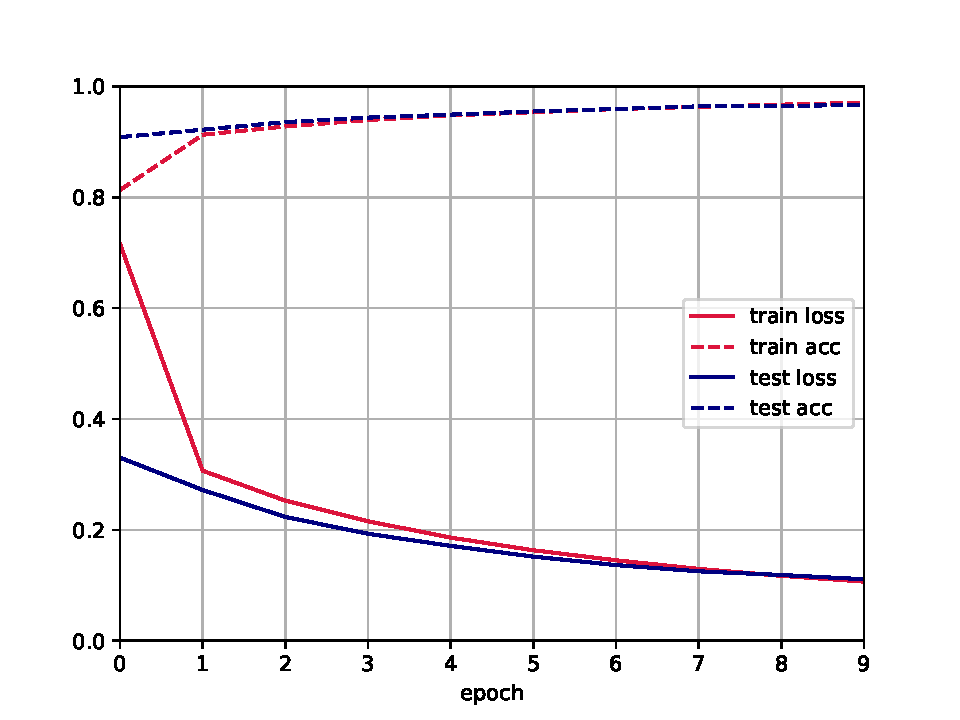
\includegraphics[width=0.7\linewidth]{hw3/final_plot.pdf}
        \caption{Caption}
        \label{fig:enter-label}
    \end{figure}

    \begin{figure}[htp]
        \centering
        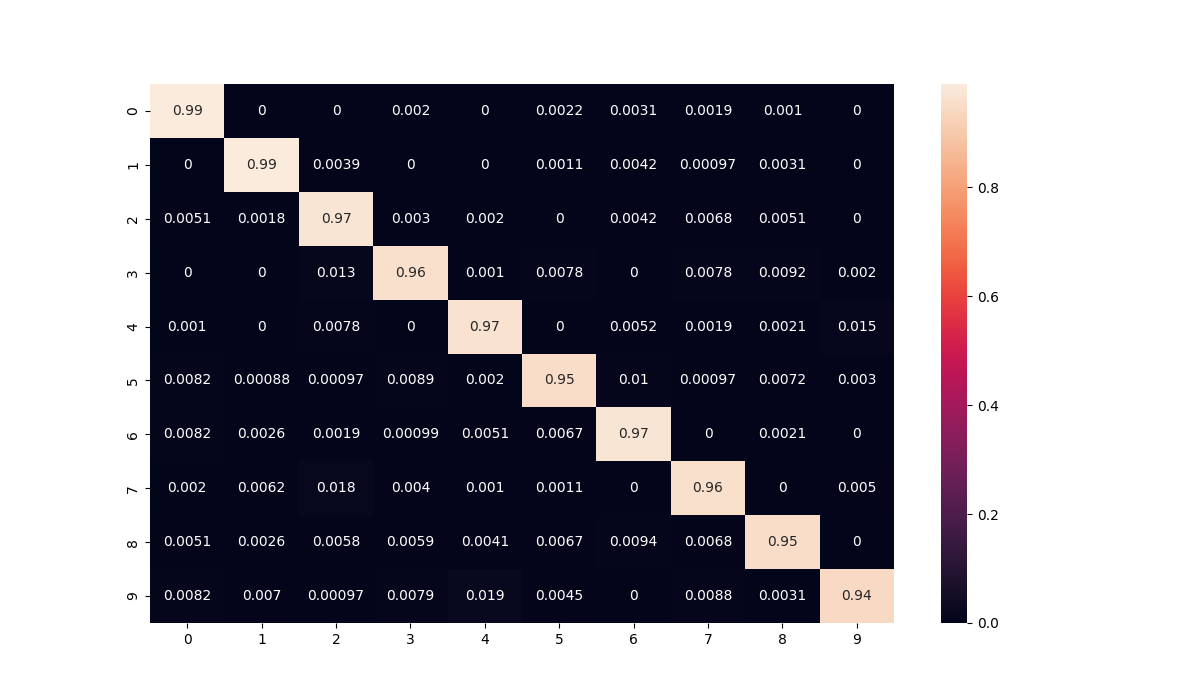
\includegraphics[width=0.7\linewidth]{hw3/confusion_matrix.png}
        \caption{Caption}
        \label{fig:enter-label}
    \end{figure}

    \item[2.] The graph illustrates the improvement of our model as the number of epochs increases. Obviously, we want to minimize loss and maximize accuracy, which we see as the model trains. That being said, the improvements slow own over time, as the parameters converge towards an optima. We can see how the training accuracy and loss start worse than test accuracy and loss. This can be due to a variety of reasons like potentially the test set being easier images to classify. That being said the important part is they converge (i.e. not training higher than loss), are improving through the epochs, and seem to be converging to optimal parameters. All 3 of these trends are visible in our graph. 

    \item[3.]

      Test Accuracy (In Distribution): 0.99632

      Test Accuracy (Out of Distribution): 0.0

      Discussion: We can clearly see the failure of the model to perform in OOD data given its accuracy of 0.0. This is in comparison to our in distribution test accuracy of 0.996. Clearly the our model is capable of performing, and it generalizes well to outside of the training data, however, it does not do well at generalizing outside the scope of the training data. Investigating the code, it becomes pretty clear as to why this is. Our model is trained on 1s, and 6s. The in distribution test set was also a set of 1s and 6s, which is why our model was able to maintain a high accuracy on it. That being said, the out of distribution dataset is 3s. The model was never trained to be able to recognize 3s and even though it is capable (i.e. its output variable is capable of predicting 3s), it will never do so, because it would not have expected a 3 given it has never 'seen' one before. 

    \item[4.] To help with this we can investigate the confusion matrix. The confusion matrix allows us to visualize where there is uncertainty in the model by seeing where it falters. With the rows being the true value, and the columns being the predicted, the values represent how often a certain true value will be mistaken for a different one. As such, the highest values represent where the model is most uncertain. Some of these examples in the confusion matrix are true 7s are often mistaken (0.018) for 2s, or a true 9 for a 4 (.019). These make sense because we can see the similarities between these numbers. A 9 written with straighter lines is similar to a 4.  These uncertainties help us understand the limitations of the model. When you receive a prediction that is a value that is often confused for another, you may want to be more hesitant as to the confidence of that value. These uncertainties are unhelpful in that they are generalized uncertainties, and are not specific to each input. We simply know that 7s are often mistaken for 2s, but not that a specific 7 will be mistaken for a 2. There is little uncertainty in the OOD model, yet it is wrong because it does not have sufficient information. In a sense, it is certain to predict a 1 or 6, but is wrong in that certainty. This because it has no idea what it is looking at when it receives a 3, but expects it to be a 1 or 6, and thus is confident in one of those predictions. Multiple training models definitely will not help for OOD model because it will always just be 3s in the dataset (if bootstrapping from that set), but will help for in distribution data because the non-edge cases will be similar across all (if not most) models, and the edge cases might be generalized out, by some models focusing more on that distinction and thus be better at that prediction. 

    \item[5.]

      \begin{enumerate}
        \item They could adjust how the scanner works, and ensure that the laser only reads a certain pattern, that is, the laser would malfunction and always receive a signal for a certain zip code as opposed to reacting to each envelope. It could also manipulate the clarity of the scanners images, so that it becomes difficult to tell the difference between certain numbers like 8 and 0. The safeguards would be generally physical. They have to ensure the adversary does not have access to the scanner, i.e. increased security and other things. It also might be helpful to add security checks every morning to ensure the scanner was not tampered with and is working correctly. The drawbacks are generally the time and money cost of adding these checks or increasing security, thus slowing down the process. 
        \item If an adversary had access to the envelopes they could simply change the inputs. If they want a certain output from the model, and have access to the envelopes then simply change what the envelope says to the input for the correlated output. Safeguards against this are again increased security to ensure the envelopes have not been tampered with. This could include sorting out ones who have had their zip codes changed and thus might need an extra level of precaution to ensure the change was not an attack on the system. Again, these are costly solutions that will make the process less efficient, but may be likely to prevent the system from failing. 
        \item The social engineering attack could rely on ensuring that the team retraining the model does not receive the correct training data to ensure the model is trained correctly, instead, maybe it will then be trained to always predict a certain zipcode. The social engineering attack could also be trying to persuade one of the workers to sabotage the model to work a specific way. To safeguard against this, you could maybe compartmentalize the model to prevent one worker from having enough control over it as to be able to cause such an effect. Ensure the data being used to train the model also is correct. The downsides are that the training of the model may slow down, as the teams are less able to work together as the project is compartmentalized. Nonetheless this may be helpful to prevent against these attacks. 

        \item **I do not understand whether this is a different question or was supposed to be grouping all together the other parts, but I will treat it as a different question** The safeguards that could be implemented, ensure the efficacy of the system as a hole, ensuring that all parts of the model, from its inputs, to the training, are using the expected data. Added costs and time to train the model and secure it may become necessary to prevent any foul-play, such as changing the zipcodes on the envelopes, or coercing the workers to manipulate the parameters, yet it becomes important to secure each element in order to prevent attacks at any level of the progression. These include but are not limited to added security workers, added security checks, and potentially compartmentalization of workload. 
      \end{enumerate}


  \end{enumerate}

\end{answer}


%%%%%%%%%%%%%%%%%%%%%%%%%%%%%%%%%%%%%%%%%%%%%
% Name and Calibration
%%%%%%%%%%%%%%%%%%%%%%%%%%%%%%%%%%%%%%%%%%%%%
\newpage
\subsection*{Name} Ethan Veghte

\subsection*{Collaborators and Resources}
Whom did you work with, and did you use any resources beyond cs181-textbook and your notes?


\end{document}
